\documentclass[12pt, twoside]{article}
\usepackage[letterpaper, margin=1in, headsep=0.5in]{geometry}
\usepackage[english]{babel}
\usepackage[utf8]{inputenc}
\usepackage{amsmath}
\usepackage{amsfonts}
\usepackage{amssymb}
\usepackage{tikz}
\usetikzlibrary{quotes, angles}
\usepackage{graphicx}
\usepackage{enumitem}
\usepackage{multicol}

\newif\ifmeta
\metatrue %print standards and topics tags

\title{Regents Geometry}
\author{Chris Huson}
\date{December 2021}

\usepackage{fancyhdr}
\pagestyle{fancy}
\fancyhf{}
\renewcommand{\headrulewidth}{0pt} % disable the underline of the header
\raggedbottom


\fancyhead[LE]{\thepage}
\fancyhead[RO]{\thepage \\ Name: \hspace{4cm} \,\\}
\fancyhead[LO]{BECA / Dr. Huson / Geometry 5 Congruence Transformations}

\begin{document}

\subsubsection*{5.2 Classwork: Reflection \hfill CCSS.HSN.RN.A.2}
\begin{enumerate}
  \item Reflect the point $A(4)$ across the origin. (flip the number line) Mark and label it $A'$.
  \begin{center}
      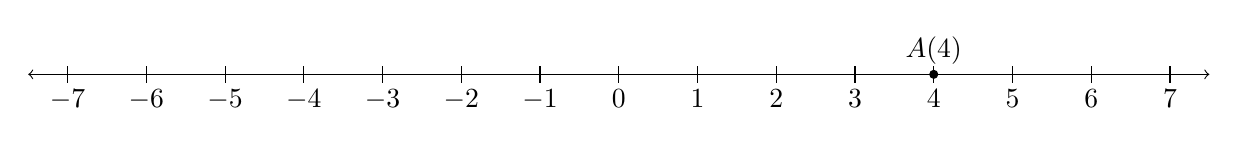
\begin{tikzpicture}
        \draw [<->] (-7.5,0)--(7.5,0);
        \foreach \x in {-7,...,7}
          \draw[shift={(\x,0)},color=black] (0pt,-3pt) -- (0pt,3pt) node[below=5pt]  {$\x$};
          \draw [fill] (4,0) circle [radius=0.05] node[above] {$A(4)$};
      \end{tikzpicture}
    \end{center}

  \item On the axes below, graph the point $P(-4,3)$ and its image, $P'$, after a reflection across the $x$-axis. Mark $P'$ and write it down as a coordinate pair.
    \begin{center}
      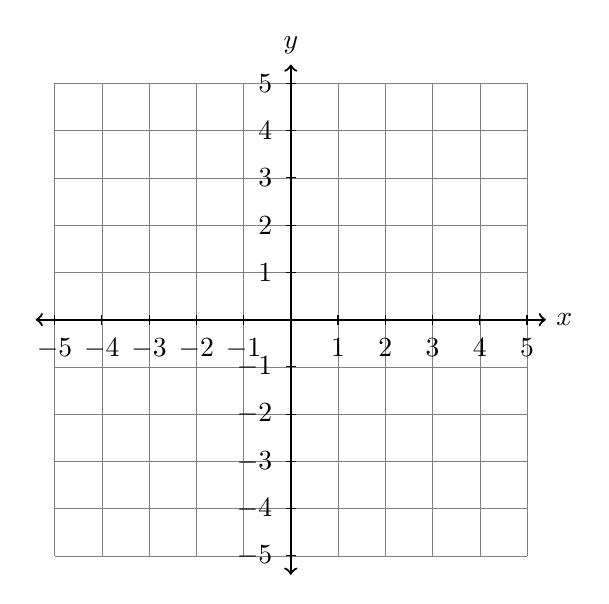
\begin{tikzpicture}[scale=.6]
      \draw [help lines] (-5,-5) grid (5,5);
      \draw [thick, <->] (-5.4,0) -- (5.4,0) node [right] {$x$};
      \draw [thick, <->] (0,-5.4)--(0,5.4) node [above] {$y$};
      \foreach \x in {-5,...,-1,1,2,3,4,5}
        \draw[shift={(\x,0)},color=black] (0pt,-3pt) -- (0pt,3pt) node[below=5pt]  {$\x$};
      \foreach \y in {-5,...,-1,1,2,3,4,5}
        \draw[shift={(0,\y)},color=black] (-3pt,0pt) -- (3pt,0pt) node[left=5pt]  {$\y$}; 
    \end{tikzpicture}
  \end{center}

\item A reflection maps $Q(4,3)$ onto $Q'(4,-3)$. Is the reflection across the $x$-axis or the $y$-axis? \vspace{1cm}

\item Reflect $\triangle JKL$ across the $y$-axis, labeling the image $\triangle J'K'L'$.
\begin{center}
    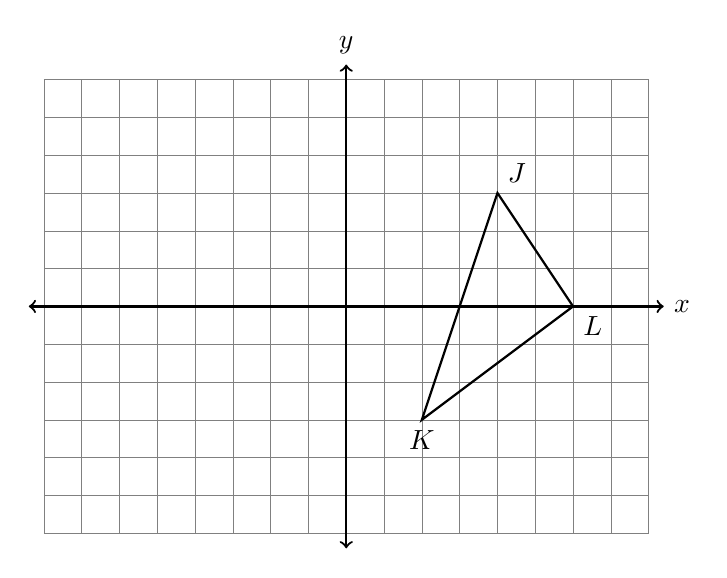
\begin{tikzpicture}[scale=.48]
    \draw [help lines] (-8,-6) grid (8,6);
    \draw [thick, <->] (-8.4,0) -- (8.4,0) node [right] {$x$};
    \draw [thick, <->] (0,-6.4)--(0,6.4) node [above] {$y$};  
    \draw [thick]
      (4,3) node[above right] {$J$}--
      (2,-3) node[below] {$K$}--
      (6,0) node[below right] {$L$}--cycle;  
  \end{tikzpicture}
\end{center}

\newpage
\item Triangle $A'B'C'$ is the image of triangle $ABC$ after a reflection. Is triangle $ABC$ congruent to $A'B'C'$? Explain why. \vspace{3cm}

\item In the graph below, a transformation maps $\triangle PQR$ onto $\triangle STU$.
\begin{multicols}{2}
  \begin{enumerate}
    \item Completely identify the transformation.
    \item What point corresponds to $T$?
    \item Is $R$ the image of $U$, or its preimage? \vspace{1cm}
  \end{enumerate}
    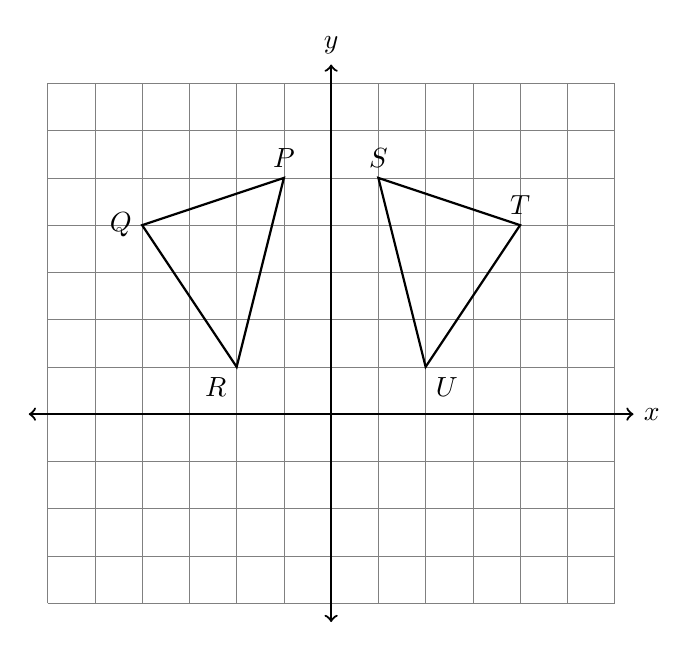
\begin{tikzpicture}[scale=.6]
    \draw [help lines] (-6,-4) grid (6,7);
    \draw [thick, <->] (-6.4,0) -- (6.4,0) node [right] {$x$};
    \draw [thick, <->] (0,-4.4)--(0,7.4) node [above] {$y$};  
    \draw [thick]
      (-1,5) node[above] {$P$}--
      (-4,4) node[left] {$Q$}--
      (-2,1) node[below left] {$R$}--cycle;
    \draw [thick]
    (1,5) node[above] {$S$}--
    (4,4) node[above] {$T$}--
    (2,1) node[below right] {$U$}--cycle;
  \end{tikzpicture}
\end{multicols}

\item In the graph below, a transformation maps $\triangle ABC \rightarrow \triangle A'B'C'$.
\begin{multicols}{2}
Angie says the triangle must have been reflected across the $y$-axis. Robbie says it might have been reflected, but it could also have been translated to the right.\\[0.25cm] 
Who is correct? Justify your answer.
    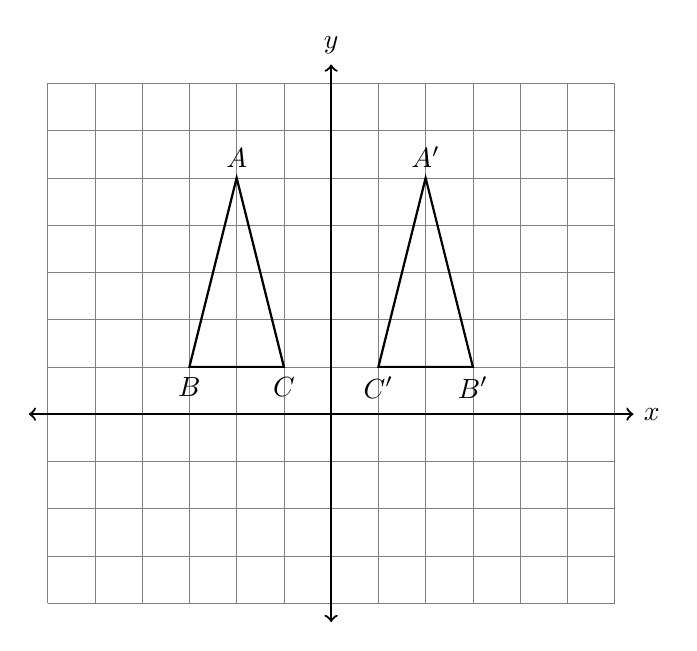
\begin{tikzpicture}[scale=.6]
    \draw [help lines] (-6,-4) grid (6,7);
    \draw [thick, <->] (-6.4,0) -- (6.4,0) node [right] {$x$};
    \draw [thick, <->] (0,-4.4)--(0,7.4) node [above] {$y$};  
    \draw [thick]
      (-2,5) node[above] {$A$}--
      (-3,1) node[below] {$B$}--
      (-1,1) node[below] {$C$}--cycle;
    \draw [thick]
    (2,5) node[above] {$A'$}--
    (3,1) node[below] {$B'$}--
    (1,1) node[below] {$C'$}--cycle;
  \end{tikzpicture}
\end{multicols}

\item Two transformations have been applied to a triangle in the diagram below, \\$\triangle ABC \rightarrow \triangle A'B'C' \rightarrow \triangle A''B''C''$. Fully characterize each transformation.
  \begin{flushright}
      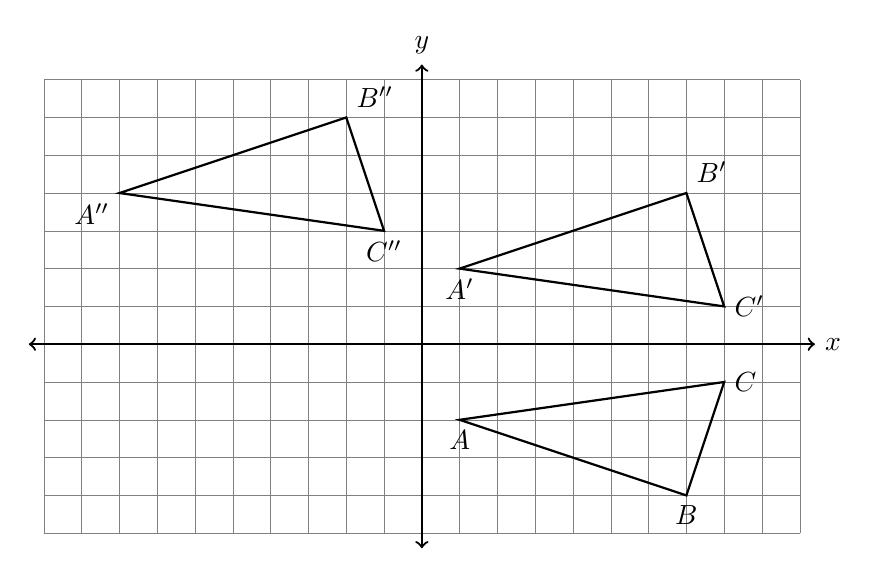
\begin{tikzpicture}[scale=.48]
      \draw [help lines] (-10,-5) grid (10,7);
      \draw [thick, <->] (-10.4,0) -- (10.4,0) node [right] {$x$};
      \draw [thick, <->] (0,-5.4)--(0,7.4) node [above] {$y$};  
      \draw [thick]
        (-8,4) node[below left] {$A''$}--
        (-2,6) node[above right] {$B''$}--
        (-1,3) node[below] {$C''$}--cycle;
      \draw [thick]
        (1,2) node[below] {$A'$}--
        (7,4) node[above right] {$B'$}--
        (8,1) node[right] {$C'$}--cycle;  
        \draw [thick]
        (1,-2) node[below] {$A$}--
        (7,-4) node[below] {$B$}--
        (8,-1) node[right] {$C$}--cycle;
    \end{tikzpicture}
  \end{flushright}

\item A reflection maps $\triangle ABC \rightarrow \triangle A'B'C'$. Which triangle has the larger area, the preimage or the image (or neither)? Justify your answer. \vspace{3cm}

\item Draw the line of reflection that would map $\triangle ABC$ onto $\triangle A'B'C'$.
\begin{center}
    \begin{tikzpicture}[rotate=-100]
    %\draw [help lines] (-7,-2) grid (7,6);
    %\draw [thick, <->] (-7.4,0) -- (7.4,0) node [right] {$x$};
    %\draw [thick, <->] (0,-2.4)--(0,6.4) node [above] {$y$};  
    \draw [thick]
      (0,2) node[left] {$A$}--
      (3,4) node[right] {$B$}--
      (-2,3) node[left] {$C$}--cycle;
    \draw [thick]
    (2,0) node[above] {$A'$}--
    (4,3) node[below left] {$B'$}--
    (3,-2) node[left] {$C'$}--cycle;
  \end{tikzpicture}
\end{center}

\newpage
\item Which of the following would map $\triangle CAT \rightarrow \triangle C'A'T'$?  \vspace{0.5cm}
  \begin{multicols}{2}
    \begin{itemize}
      \item[T \quad F \quad] Reflected across the $y$-axis
      \item[T \quad F \quad] Translated six to the left, down zero
      \item[T \quad F \quad] Reflected across the $y$-axis, then slid to the left two
      \item[T \quad F \quad] $(x,y) \rightarrow (x-6, y+0)$
      %\item[T \quad F \quad] Rotated $90^\circ$ counterclockwise around the origin
      \item[T \quad F \quad] Reflected across the line $x=-1$
    \end{itemize}
    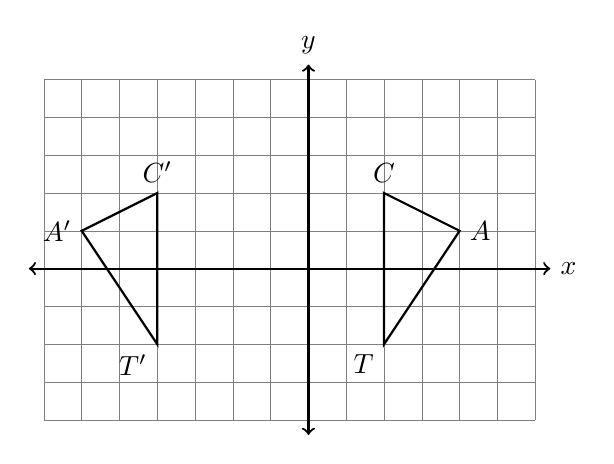
\begin{tikzpicture}[scale=.48]
      \draw [help lines] (-7,-4) grid (6,5);
      \draw [thick, <->] (-7.4,0) -- (6.4,0) node [right] {$x$};
      \draw [thick, <->] (0,-4.4)--(0,5.4) node [above] {$y$};  
      \draw [thick]
      (2,2) node[above] {$C$}--
      (4,1) node[right] {$A$}--
      (2,-2) node[below left] {$T$}--cycle;
      \draw [thick]
      (-4,2) node[above] {$C'$}--
      (-6,1) node[left] {$A'$}--
      (-4,-2) node[below left] {$T'$}--cycle;
    \end{tikzpicture}
  \end{multicols}

\item Draw the line of reflection for quadrilaterals in the diagram below.
  \begin{center}
  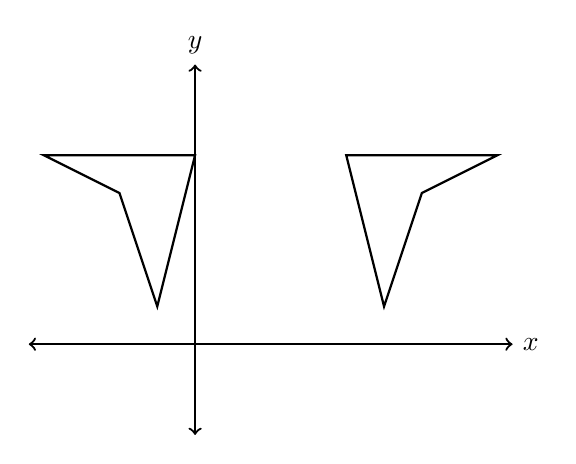
\begin{tikzpicture}[scale=.48]
    %\draw [help lines] (-10,-7) grid (10,7);
    \draw [thick, <->] (-4.4,0) -- (8.4,0) node [right] {$x$};
    \draw [thick, <->] (0,-2.4)--(0,7.4) node [above] {$y$};  
    \draw [thick](5,1)--(6,4)--(8,5)--(4,5)--cycle;  
    \draw [thick](-1,1)--(-2,4)--(-4,5)--(0,5)--cycle;
  \end{tikzpicture}
\end{center}

\item First reflect the trapezoid $BECA$ across the $x$-axis, then move it down 1 and right 7. Label the images $B'E'C'A'$ and $B''E''C''A''$.
  \begin{center}
      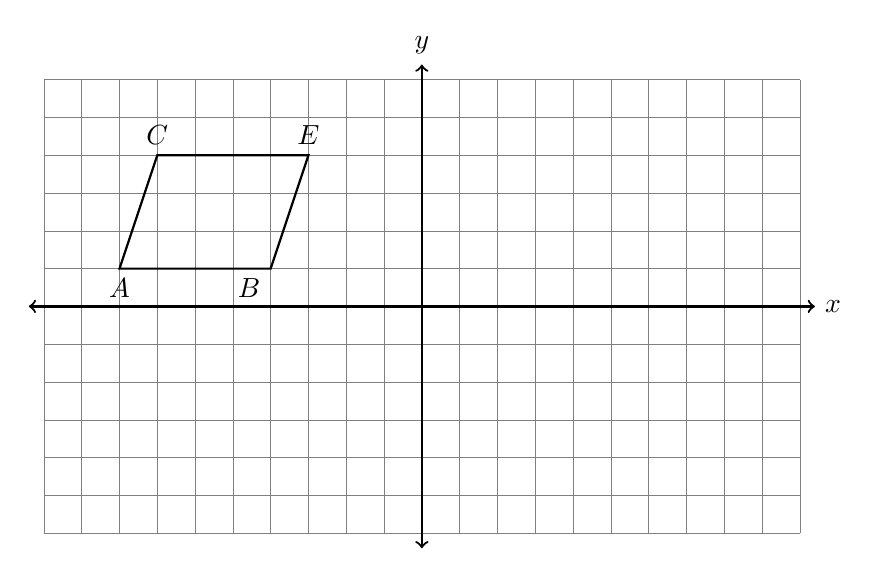
\begin{tikzpicture}[scale=.48]
      \draw [help lines] (-10,-6) grid (10,6);
      \draw [thick, <->] (-10.4,0) -- (10.4,0) node [right] {$x$};
      \draw [thick, <->] (0,-6.4)--(0,6.4) node [above] {$y$};  
      \draw [thick]
        (-4,1) node[below left] {$B$}--
        (-3,4) node[above] {$E$}--
        (-7,4) node[above] {$C$}--
        (-8,1) node[below] {$A$}--cycle;  
    \end{tikzpicture}
  \end{center}

\newpage
  \item The quadrilateral $ROCK$ undergoes rigid motions, shown below. Describe the sequence of transformations applied.
  \begin{flushright}
      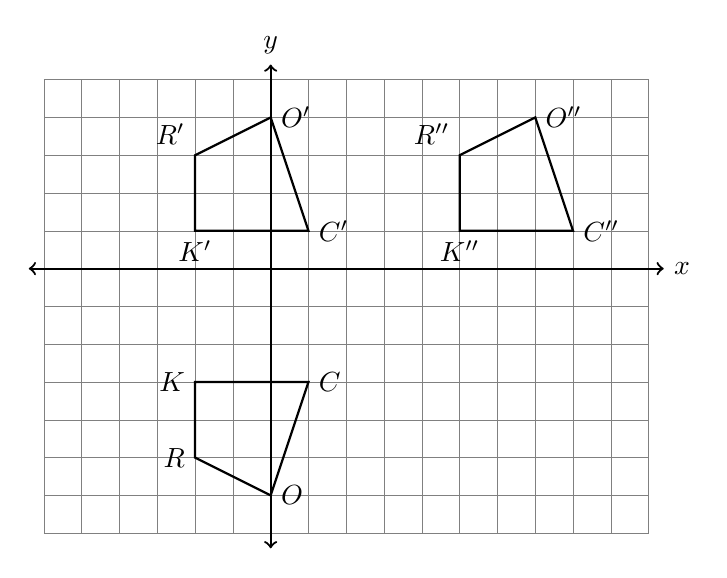
\begin{tikzpicture}[scale=.48]
      \draw [help lines] (-6,-7) grid (10,5);
      \draw [thick, <->] (-6.4,0) -- (10.4,0) node [right] {$x$};
      \draw [thick, <->] (0,-7.4)--(0,5.4) node [above] {$y$};  
      \draw [thick]
        (5,1) node[below] {$K''$}--
        (5,3) node[above left] {$R''$}--
        (7,4) node[right] {$O''$}--
        (8,1) node[right] {$C''$}--cycle;
      \draw [thick]
        (-2,1) node[below] {$K'$}--
        (-2,3) node[above left] {$R'$}--
        (0,4) node[right] {$O'$}--
        (1,1) node[right] {$C'$}--cycle;  
      \draw [thick]
      (-2,-3) node[left] {$K$}--
      (-2,-5) node[left] {$R$}--
      (0,-6) node[right] {$O$}--
      (1,-3) node[right] {$C$}--cycle;
    \end{tikzpicture}
  \end{flushright}

  \item The quadrilateral $MATH$ is mapped to $M'A'T'H'$ by a rigid motion. What transformation a been applied?  \vspace{0.5cm}
  \begin{multicols}{2}
    \begin{enumerate}
      \item Dilation
      \item Reflection
      \item Rotation
      \item Translation
    \end{enumerate}
    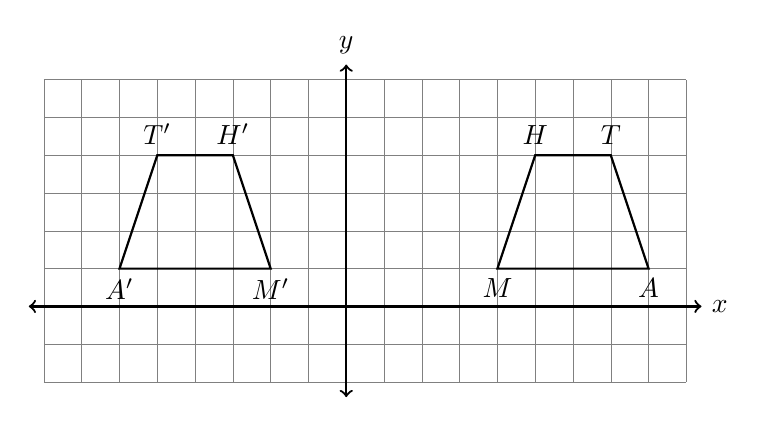
\begin{tikzpicture}[scale=.48]
      \draw [help lines] (-8,-2) grid (9,6);
      \draw [thick, <->] (-8.4,0) -- (9.4,0) node [right] {$x$};
      \draw [thick, <->] (0,-2.4)--(0,6.4) node [above] {$y$};  
      \draw [thick]
        (4,1) node[below] {$M$}--
        (8,1) node[below] {$A$}--
        (7,4) node[above] {$T$}--
        (5,4) node[above] {$H$}--cycle;
      \draw [thick]
        (-2,1) node[below] {$M'$}--
        (-6,1) node[below] {$A'$}--
        (-5,4) node[above] {$T'$}--
        (-3,4) node[above] {$H'$}--cycle; 
    \end{tikzpicture}
  \end{multicols}

\newpage
  \item Given $\triangle WIN \cong \triangle W'I'N'$. Describe the rigid motion mapping $\triangle WIN \rightarrow \triangle W'I'N'$.
  \begin{flushright}
    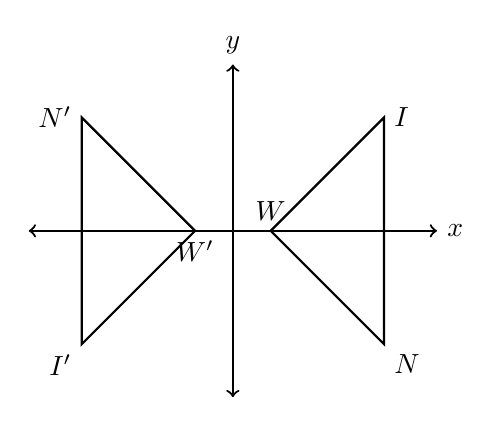
\begin{tikzpicture}[scale=.48]
      %\draw [help lines] (-10,-7) grid (10,7);
      \draw [thick, <->] (-5.4,0) -- (5.4,0) node [right] {$x$};
      \draw [thick, <->] (0,-4.4)--(0,4.4) node [above] {$y$};  
      \draw [thick]
      (1,0) node[above] {$W$}--
      (4,3) node[right] {$I$}--
      (4,-3) node[below right] {$N$}--cycle;
      \draw [thick]
      (-1,0) node[below] {$W'$}--
      (-4,3) node[left] {$N'$}--
      (-4,-3) node[below left] {$I'$}--cycle;
    \end{tikzpicture}
  \end{flushright}

  \item Determine and state the sequence of transfromations applied to map $BECA$ to $B''E''C''A''$.
  \begin{flushright}
      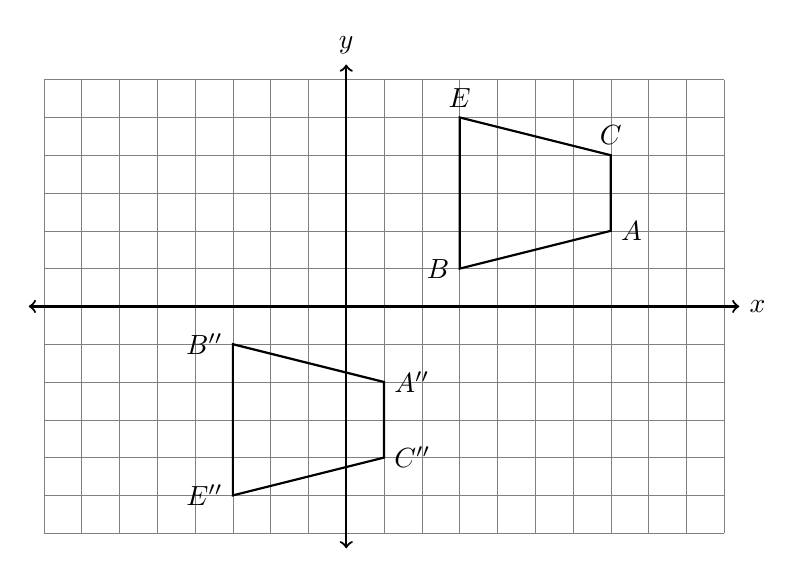
\begin{tikzpicture}[scale=.48]
      \draw [help lines] (-8,-6) grid (10,6);
      \draw [thick, <->] (-8.4,0) -- (10.4,0) node [right] {$x$};
      \draw [thick, <->] (0,-6.4)--(0,6.4) node [above] {$y$};  
      \draw [thick]
        (3,1) node[left] {$B$}--
        (3,5) node[above] {$E$}--
        (7,4) node[above] {$C$}--
        (7,2) node[right] {$A$}--cycle;
      \draw [thick]
        (-3,-1) node[left] {$B''$}--
        (-3,-5) node[left] {$E''$}--
        (1,-4) node[right] {$C''$}--
        (1,-2) node[right] {$A''$}--cycle; 
    \end{tikzpicture}
  \end{flushright}

  \item Determine and state the transformation mapping $\triangle NOP$ onto $\triangle QRP$. 
    \begin{flushright}
        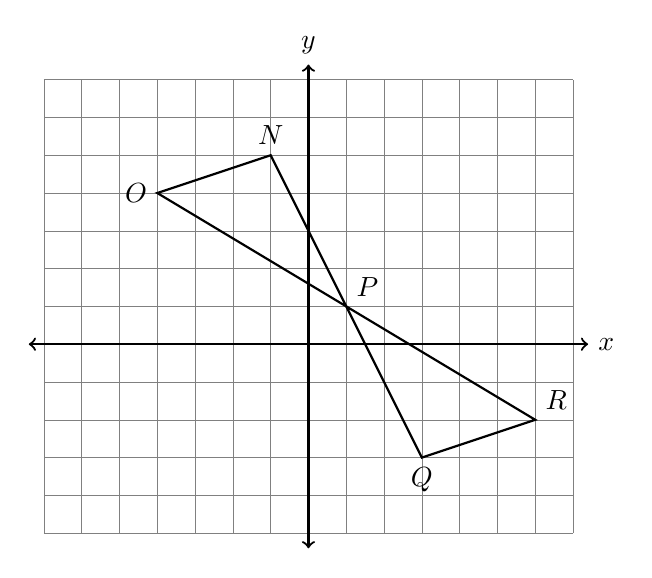
\begin{tikzpicture}[scale=.48]
        \draw [help lines] (-7,-5) grid (7,7);
        \draw [thick, <->] (-7.4,0) -- (7.4,0) node [right] {$x$};
        \draw [thick, <->] (0,-5.4)--(0,7.4) node [above] {$y$};  
        \draw [thick]
          (-1,5) node[above] {$N$}--
          (-4,4) node[left] {$O$}--
          (1,1) --cycle;
        \draw [thick]
        (3,-3) node[below] {$Q$}--
        (6,-2) node[above right] {$R$}--
        (1,1) node[above right] {$P$}--cycle;
      \end{tikzpicture}
    \end{flushright}

\end{enumerate}
\end{document}